% =====================================================================
% Fig. 4 - Frequency-Aware Branch Gating (FEATHer module [3]).
%
% Zoom-in of Fig.1 module [3]. The figure traces the gate-weight
% computation through five intermediate visualisations:
%
%   X tilde  ->  FFT magnitude  ->  channel-mean spectrum
%            ->  Conv1D (4-band reducer) -> freq-mean (4 scalars)
%            ->  softmax -> 4 gate weights (one per branch).
%
% Shared palette with Fig.1 / Fig.2 (pointC/highC/midC/lowC) so the
% four bars at the right map directly to the four DTK branches that
% the gate weights are applied to in the main architecture.
% =====================================================================
\documentclass[tikz, border=8pt]{standalone}

\usepackage{amsmath, amssymb}
\usepackage{tikz}
\usetikzlibrary{arrows.meta, positioning, calc, decorations.pathreplacing}

\definecolor{pointC}{HTML}{6B7280}
\definecolor{highC}{HTML}{DC2626}
\definecolor{midC}{HTML}{F59E0B}
\definecolor{lowC}{HTML}{2563EB}
\definecolor{specC}{HTML}{EA580C}      % orange for spectra

\begin{document}

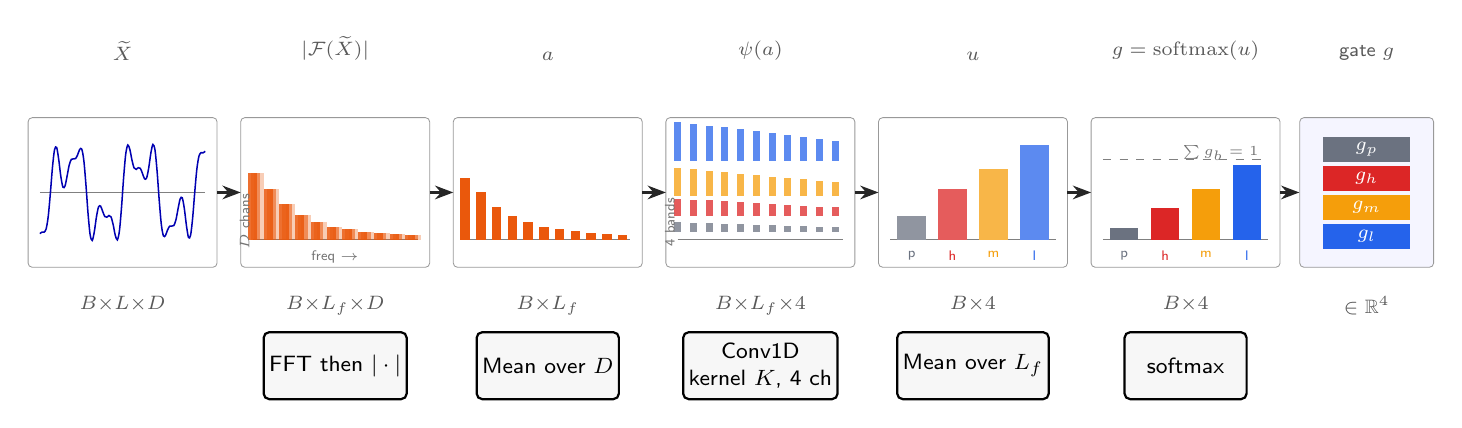
\begin{tikzpicture}[
    font=\sffamily\small,
    >=Stealth,
    op/.style={
        draw, thick,
        rounded corners=2pt,
        fill=gray!6,
        minimum width=1.55cm,
        minimum height=0.85cm,
        align=center,
        font=\sffamily\footnotesize,
        inner sep=2pt
    },
    panel/.style={
        draw=black!40, line width=0.3pt,
        rounded corners=1.5pt,
        fill=white
    },
    flow/.style={->, thick, draw=black!85},
    axis/.style={draw=black!50, line width=0.3pt},
    caption/.style={font=\sffamily\scriptsize, text=black!65}
]

% =====================================================================
% Pipeline geometry (panel width 2.4cm, spacing 2.7cm => 0.3cm gap)
% =====================================================================
\def\xIn{0}
\def\xFFT{2.7}
\def\xMeanD{5.4}
\def\xConv{8.1}
\def\xMeanL{10.8}
\def\xSoft{13.5}
\def\xOut{15.8}

% panel dims
\def\pW{1.20}      % visualisation panel half-width
\def\pH{0.95}      % visualisation panel half-height
\def\opYoff{-2.2}  % operator block sits below panel
\def\labYoff{ 1.55} % data label sits above panel

% =====================================================================
% 1. Input: time-domain waveform
% =====================================================================
\node[panel, minimum width={2*\pW cm}, minimum height={2*\pH cm}] (P1) at (\xIn, 0) {};
\node[caption, anchor=south] at (\xIn, \labYoff) {$\widetilde{X}$};
\begin{scope}[shift={(\xIn, 0)}]
    \draw[axis] (-\pW + 0.15, 0) -- (\pW - 0.15, 0);
    \draw[blue!70!black, line width=0.55pt, smooth, samples=80,
          domain={-\pW + 0.15}:{\pW - 0.15}]
        plot (\x, {0.45*sin(7*\x r) + 0.3*sin(20*\x r) + 0.15*sin(35*\x r)});
\end{scope}

% =====================================================================
% 2. FFT magnitude: spectrum bars with channel multiplicity (3 layers)
% =====================================================================
\node[panel, minimum width={2*\pW cm}, minimum height={2*\pH cm}] (P2) at (\xFFT, 0) {};
\node[caption, anchor=south] at (\xFFT, \labYoff) {$|\mathcal{F}(\widetilde X)|$};
\begin{scope}[shift={(\xFFT, 0)}]
    \draw[axis] (-\pW + 0.15, -0.6) -- (\pW - 0.15, -0.6);
    % 3 stacked channels (D dimension) - all 3 spectra drawn lightly with small shift
    \foreach \dy/\op in {0.10/30, 0.05/55, 0.00/85} {
        \foreach \bxR/\bh in {-1.05/0.85, -0.85/0.65, -0.65/0.45, -0.45/0.32, -0.25/0.22,
                             -0.05/0.16, 0.15/0.13, 0.35/0.10, 0.55/0.08, 0.75/0.07, 0.95/0.06} {
            \pgfmathsetmacro{\bx}{\bxR + \dy * 0.8}
            \fill[specC, opacity=\op/100]
                (\bx - 0.06, -0.6) rectangle (\bx + 0.06, -0.6 + \bh);
        }
    }
    \node[font=\sffamily\tiny, text=black!55, anchor=north]
        at (0, -0.62) {freq $\to$};
    \node[font=\sffamily\tiny, text=black!55, anchor=east, rotate=90]
        at (-\pW + 0.05, 0.1) {$D$ chans};
\end{scope}

% =====================================================================
% 3. Channel-mean spectrum (single curve / single bar set)
% =====================================================================
\node[panel, minimum width={2*\pW cm}, minimum height={2*\pH cm}] (P3) at (\xMeanD, 0) {};
\node[caption, anchor=south] at (\xMeanD, \labYoff) {$a$};
\begin{scope}[shift={(\xMeanD, 0)}]
    \draw[axis] (-\pW + 0.15, -0.6) -- (\pW - 0.15, -0.6);
    \foreach \bx/\bh in {-1.05/0.78, -0.85/0.60, -0.65/0.42, -0.45/0.30, -0.25/0.22,
                         -0.05/0.16, 0.15/0.13, 0.35/0.11, 0.55/0.09, 0.75/0.07, 0.95/0.06} {
        \fill[specC] (\bx - 0.06, -0.6) rectangle (\bx + 0.06, -0.6 + \bh);
    }
\end{scope}

% =====================================================================
% 4. Conv1D output: 4-channel feature spectrum, lightly colored per band
% =====================================================================
\node[panel, minimum width={2*\pW cm}, minimum height={2*\pH cm}] (P4) at (\xConv, 0) {};
\node[caption, anchor=south] at (\xConv, \labYoff) {$\psi(a)$};
\begin{scope}[shift={(\xConv, 0)}]
    \draw[axis] (-\pW + 0.15, -0.6) -- (\pW - 0.15, -0.6);
    % four lanes each as a thin colored bar series at different heights
    \def\xL{-1.05}
    \def\xStep{0.20}
    \foreach \cy/\cc/\hpat in {%
        0.40/lowC/0.50,
       -0.05/midC/0.36,
       -0.30/highC/0.22,
       -0.50/pointC/0.12%
    } {
        \foreach \i in {0,1,...,10} {
            \pgfmathsetmacro{\bx}{\xL + \i * \xStep}
            \pgfmathsetmacro{\hh}{\hpat * (1 - 0.05*\i)}
            \fill[\cc!75] (\bx - 0.045, \cy) rectangle (\bx + 0.045, \cy + \hh);
        }
    }
    \node[font=\sffamily\tiny, text=black!55, anchor=east, rotate=90]
        at (-\pW + 0.05, 0.05) {4 bands};
\end{scope}

% =====================================================================
% 5. Mean over L_f: 4 scalars (one per band)
% =====================================================================
\node[panel, minimum width={2*\pW cm}, minimum height={2*\pH cm}] (P5) at (\xMeanL, 0) {};
\node[caption, anchor=south] at (\xMeanL, \labYoff) {$u$};
\begin{scope}[shift={(\xMeanL, 0)}]
    \draw[axis] (-\pW + 0.15, -0.6) -- (\pW - 0.15, -0.6);
    % 4 thicker bars (pre-softmax logits, can be uneven heights)
    \def\bW{0.18}
    \fill[pointC!75] (-0.78 - \bW, -0.6) rectangle (-0.78 + \bW, -0.6 + 0.30);
    \fill[highC!75]  (-0.26 - \bW, -0.6) rectangle (-0.26 + \bW, -0.6 + 0.65);
    \fill[midC!75]   ( 0.26 - \bW, -0.6) rectangle ( 0.26 + \bW, -0.6 + 0.90);
    \fill[lowC!75]   ( 0.78 - \bW, -0.6) rectangle ( 0.78 + \bW, -0.6 + 1.20);
    \node[font=\sffamily\tiny, text=pointC, anchor=north] at (-0.78, -0.62) {p};
    \node[font=\sffamily\tiny, text=highC,  anchor=north] at (-0.26, -0.62) {h};
    \node[font=\sffamily\tiny, text=midC,   anchor=north] at ( 0.26, -0.62) {m};
    \node[font=\sffamily\tiny, text=lowC,   anchor=north] at ( 0.78, -0.62) {l};
\end{scope}

% =====================================================================
% 6. Softmax: 4 normalised gate weights (summing to 1)
% =====================================================================
\node[panel, minimum width={2*\pW cm}, minimum height={2*\pH cm}] (P6) at (\xSoft, 0) {};
\node[caption, anchor=south] at (\xSoft, \labYoff) {$g = \mathrm{softmax}(u)$};
\begin{scope}[shift={(\xSoft, 0)}]
    \draw[axis] (-\pW + 0.15, -0.6) -- (\pW - 0.15, -0.6);
    \def\bW{0.18}
    % softmaxed: heights illustrative (sum=1) e.g. 0.10, 0.20, 0.30, 0.40
    \fill[pointC] (-0.78 - \bW, -0.6) rectangle (-0.78 + \bW, -0.6 + 0.15);
    \fill[highC]  (-0.26 - \bW, -0.6) rectangle (-0.26 + \bW, -0.6 + 0.40);
    \fill[midC]   ( 0.26 - \bW, -0.6) rectangle ( 0.26 + \bW, -0.6 + 0.65);
    \fill[lowC]   ( 0.78 - \bW, -0.6) rectangle ( 0.78 + \bW, -0.6 + 0.95);
    % dashed line for "sum=1" budget
    \draw[black!50, dashed, line width=0.3pt]
        (-\pW + 0.15, 0.42) -- (\pW - 0.15, 0.42);
    \node[font=\sffamily\tiny, text=black!55, anchor=east] at (\pW - 0.15, 0.50) {$\sum g_b = 1$};
    \node[font=\sffamily\tiny, text=pointC, anchor=north] at (-0.78, -0.62) {p};
    \node[font=\sffamily\tiny, text=highC,  anchor=north] at (-0.26, -0.62) {h};
    \node[font=\sffamily\tiny, text=midC,   anchor=north] at ( 0.26, -0.62) {m};
    \node[font=\sffamily\tiny, text=lowC,   anchor=north] at ( 0.78, -0.62) {l};
\end{scope}

% =====================================================================
% 7. Output gate weights g (small endcap)
% =====================================================================
\node[panel, minimum width=1.7cm, minimum height={2*\pH cm}, fill=blue!4] (P7) at (\xOut, 0) {};
\node[caption, anchor=south] at (\xOut, \labYoff) {gate $g$};
\begin{scope}[shift={(\xOut, 0)}]
    % 4 stacked colored cells representing g as a vector
    \def\cH{0.32}
    \foreach \cy/\cc/\lab in {0.55/pointC/$g_p$, 0.18/highC/$g_h$, -0.19/midC/$g_m$, -0.56/lowC/$g_l$} {
        \fill[\cc] (-0.55, \cy - \cH/2) rectangle (0.55, \cy + \cH/2);
        \node[font=\sffamily\scriptsize, text=white] at (0, \cy) {\lab};
    }
\end{scope}
\node[caption, anchor=north] at (\xOut, -\pH - 0.25) {$\in \mathbb{R}^{4}$};

% =====================================================================
% Operator boxes (below each visualisation), naming the transformation.
% =====================================================================
\node[op] (Op1) at (\xFFT, \opYoff) {FFT then $|\cdot|$};
\node[op] (Op2) at (\xMeanD, \opYoff) {Mean over $D$};
\node[op] (Op3) at (\xConv, \opYoff) {Conv1D\\ kernel $K$, 4 ch};
\node[op] (Op4) at (\xMeanL, \opYoff) {Mean over $L_f$};
\node[op] (Op5) at (\xSoft, \opYoff) {softmax};

% =====================================================================
% Pipeline arrows (panel-to-panel along x axis)
% =====================================================================
\draw[flow] (\xIn + \pW, 0)    -- (\xFFT - \pW, 0);
\draw[flow] (\xFFT + \pW, 0)   -- (\xMeanD - \pW, 0);
\draw[flow] (\xMeanD + \pW, 0) -- (\xConv - \pW, 0);
\draw[flow] (\xConv + \pW, 0)  -- (\xMeanL - \pW, 0);
\draw[flow] (\xMeanL + \pW, 0) -- (\xSoft - \pW, 0);
\draw[flow] (\xSoft + \pW, 0)  -- (P7.west);

% =====================================================================
% Tensor-shape tags below the arrows
% =====================================================================
\node[caption, anchor=north] at (\xIn, -\pH - 0.25) {$B {\times} L {\times} D$};
\node[caption, anchor=north] at (\xFFT, -\pH - 0.25) {$B {\times} L_f {\times} D$};
\node[caption, anchor=north] at (\xMeanD, -\pH - 0.25) {$B {\times} L_f$};
\node[caption, anchor=north] at (\xConv, -\pH - 0.25) {$B {\times} L_f {\times} 4$};
\node[caption, anchor=north] at (\xMeanL, -\pH - 0.25) {$B {\times} 4$};
\node[caption, anchor=north] at (\xSoft, -\pH - 0.25) {$B {\times} 4$};

\end{tikzpicture}

\end{document}
